\documentclass[12pt,a4paper]{article}
\usepackage{cmap}
\usepackage{amsmath}
\usepackage{amsfonts}
\usepackage{mathtext}
\usepackage{titlesec}

\usepackage[utf8]{inputenc}
\usepackage[T2A]{fontenc}
\usepackage{wrapfig}
\usepackage[english, russian]{babel}
\usepackage[left=2cm,right=2cm,top=2cm,bottom=2cm]{geometry}
\usepackage{indentfirst}

\DeclareSymbolFont{T2Aletters}{T2A}{cmr}{m}{it}

%%% Работа с картинками
\usepackage{graphicx}  % Для вставки рисунков
\graphicspath{{imgs/}}  % папки с картинками

\usepackage{caption}
\captionsetup{labelsep=period, labelfont=bf}

\titleformat{\section}[block]
{\normalfont}{\thesection.}{0 cm}{}
\titleformat{\subsection}[block]
{\bfseries}{\thesubsection.}{0 cm}{}

\titlespacing{\section}{17pt}{14pt}{10pt}
\titlespacing{\subsection}{17pt}{14pt}{4pt}

\def \TITLE {Отчет о выполнении лабораторной работы №1.2.3}
\def \SUBTITLE {Определение моментов инерции твердых тел с помощью трифилярного подвеса}
\def \AUTHOR {Выполнил студент группы Б03-405\\ Тимохин Даниил}
\def \DATE {4 декабря 2024 г.}

\begin{document}

\begin{titlepage}
	\centering
	\vspace{5cm}
	{\scshape\large Московский физико-технический институт \\
	(НАЦИОНАЛЬНЫЙ ИССЛЕДОВАТЕЛЬСКИЙ УНИВЕРСИТЕТ)}
	
	\vspace{4cm}
	{\LARGE \TITLE}
	
	\vspace{1cm}
	{\Huge\bf \SUBTITLE }
	
	\vspace{1cm}
	\vfill
	
\begin{flushright}
	{\LARGE \AUTHOR}
\end{flushright}
	

	\vfill

	\DATE
\end{titlepage}

\newpage

\fontsize{12}{14}\selectfont

\section{ Аннотация}
В работе измеряются моменты инерции твердых тел с помощью трифилярного подвеса. Сравниваются с моментом инерции, вычисленным по теоретическим формулам. Проверяется справедливость теоремы Гюгенса-Штейнера, а также аддитивность моментов инерции. 

\section{ Теоретическая справка}

\begin{wrapfigure}{r}{0.4\textwidth}
    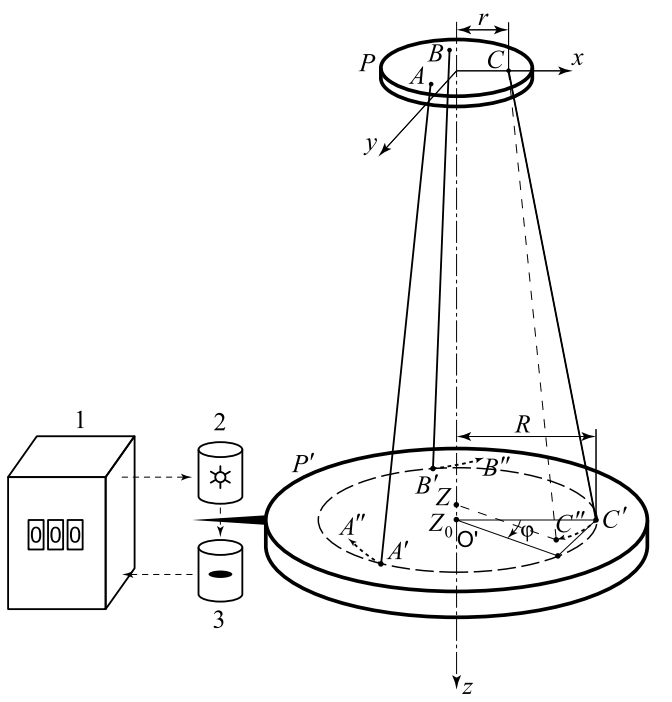
\includegraphics[width=0.4\textwidth]{imgs/ustan.png}
    \caption{Трифилярный подвес}
    \label{fig:ust1}
\end{wrapfigure}
В данной работе используется трифилярный подвес. С его помощью можно определить момент инерции, тела, расположенного на нём.

При этом энергию подвеса с грузом можно оценить так:
\begin{equation}
    \frac{I\dot{\varphi}^2}{2}+mg(z_0-z)=E
\end{equation}

Первое слагаемое - энергия вращательного движения, а второе - потенциальная энергия. Потери на трение в креплениях и неупругие деформации в нитях мы не учитываем. Считаем, что потери энергии небольшие при небольшом количестве колебаний.

Теперь запишем длину нити $CC'$ от угла поворота $\varphi$. 
\begin{equation}
    (R\cos{\varphi}-r)^2+R^2\sin^2{\varphi}+z^2=L^2
\end{equation}

И так как угол $\varphi$ мал, то можно считать $\cos{\varphi}=1-\frac{\varphi^2}{2}$
\begin{equation}
    z^2=L^2+R^2+r^2+2Rr\cos{\varphi}=z^2_0+2Rr(1-\cos{\varphi})\approx
    z^2_0-Rr\varphi^2
\end{equation}

\begin{equation}
    z^2\approx \sqrt{z^2_0-Rr\varphi^2}=z_0\sqrt{1-\frac{Rr\varphi^2}{z_0^2}} \approx z_0-\frac{Rr\varphi^2}{2z_0}
\end{equation}

В итоге получем, что 
\begin{equation}
    \frac{I\dot{\varphi}^2}{2}+mg\frac{Rr\varphi^2}{2z_0}=E
\end{equation}

Берём первую производную c учётом, что мы пренебрегаем потерями энергии
\begin{equation}
    I\ddot{\varphi}+mg\frac{Rr\varphi}{z_0}=0
\end{equation}

Получаем, что период колебаний трифилярного подвеса с грузом равен
\begin{equation}
   T=2\pi\sqrt{\frac{Iz_0}{mgRr}}
\end{equation}

Тогда для момена инерции получаем
\begin{equation}
   I=\frac{mgRrT^2}{4\pi^2z_0}
\end{equation}

\begin{equation}
   I=kmT^2,~где~k=\frac{gRr}{4\pi^2z_0}
\end{equation}
 и k - константа для установки

\section{ Оборудование}

{\bfseries Трифилярный подвес}

{\bfseries Автоматический таймер}

{\bfseries Брус}

{\bfseries Кольцо}

{\bfseries Диск}

{\bfseries Два полуцилндра(сыр)}

\section{ Результаты измерений и обработка данных}
Измерение проходит так: На подвес ставится изучаемы образец. Затем нужно сделать так, чтобы трифилярный подвес почти не совершал колебаний. Тогда можно нажать специальную кнопку для раскрутки подвеса. И с помощью специального таймера замеряем время.

Так как у таймера абсолютная и систематическая погрешность практически равна 0, то будем проводить два измерения времени и считать систематическую погрешность двух измерений.

Сначала измерим пустой подвес и посмотрим, когда амплитуда колебаний начнёт уменьшаться. Это соответствует 15 колебаниям.

Теперь сделаем измерение подвеса в 15 колебаний. Получим $T=4.42\pm0.01$ c. И измеримдлину нити подвеса.

Значение k, полученное с помощью длины нити подвеса. $k=(406.4\pm7.6)\cdot10^{-6}~\frac{м^2}{с^2}$ 

Значение $I = (7.8\pm0.14)\cdot10^{-3}~кг\cdotм^2$, а по формулам $I = (7.6812\pm0.0007)\cdot10^{-3}~кг\cdotм^2$.

Видно, что экспериментальный момент инерции соответствует теоретическому. Поэтму возьмём далее $k=(400.2\pm3.6)\cdot10^{-6}~\frac{м^2}{с^2}$.

\begin{table}[!ht]
    \caption{Полученные моменты инерции}
    \centering    
    \begin{tabular}{|c|c|c|}
    \hline
        Предметы & $T, c$ & $I,~10^{-3}~кг\cdotм^2$ \\ \hline
Подвес & $4.418 \pm 0.002 $ & $7.68 \pm 0.08 $ \\ \hline
Подвес+Кольцо & $4.1850 \pm 0.0008 $ & $12.34 \pm 0.11 $ \\ \hline
Подвес+Диск & $3.9513 \pm 0.0007 $ & $9.79 \pm 0.09 $ \\ \hline
Подвес+Брус & $3.7620 \pm 0.0005 $ & $12.36 \pm 0.11 $ \\ \hline
Подвес+Кольцо+Диск & $3.9227 \pm 0.0026 $ & $14.44 \pm 0.15 $ \\ \hline
Подвес+Брус+Диск & $3.6020 \pm 0.0016 $ & $14.37 \pm 0.14 $ \\ \hline
Подвес+Брус+Кольцо & $3.783 \pm 0.003 $ & $16.95 \pm 0.19 $ \\ \hline
    \end{tabular}
\end{table}

Проверим аддетивность фомулой $\Delta I = I_{подвес+тело1+тело2}-I_{подвес}-(I_{тело1}+I_{тело2})$

\begin{table}[!ht]
    \centering
    \caption{Проверка аддитивности момента инерции}
    \begin{tabular}{|c|c|c|}
    \hline
        Предметы & $\Delta I,~10^{-3}~кг\cdotм^2$ & $\sigma_{\Delta I},~10^{-3}~кг\cdotм^2$ \\ \hline
        Кольцо+Диск & $0.108$ & $0.200$ \\ \hline
        Брус+Диск & $0.065$ & $0.244$ \\ \hline
        Брус+Кольцо & $0.013$ & $0.211$ \\ \hline
    \end{tabular}
\end{table}

Видим, что $\Delta I$ меньше погрешности, а значит аддативность моментов инерции выполняется.

Сравним моменты инерции тел с теоретическими

\begin{equation}
    I_{Кольцо}=mr^2~~~I_{Диск}=\frac{mr^2}{2}~~~I_{Брус}=\frac{m(l^2+d^2)}{12}
\end{equation}

\begin{table}[!ht]
    \caption{Сравнения экспериментальных моментов инерции с теоретически расчитанных}
    \centering    
    \begin{tabular}{|c|c|c|}
    \hline
        Предметы & $I_{теор},~10^{-3}~кг\cdotм^2$ & $I,~10^{-3}~кг\cdotм^2$ \\ \hline
        Кольцо & 4.74 & $4.66 \pm 0.11 $ \\ \hline
        Диск & 2.12 & $2.11 \pm 0.09 $ \\ \hline
        Брус  & 4.52 & $4.68 \pm 0.11 $ \\ \hline
    \end{tabular}
\end{table}

Получаем, что измеренные нами моменты сил совпадают с теоретической оценкой.

Теперь проверим выполнение теоремы Гюгенса-Штейнера. Для этого положим два поуцилиндра в центр и будем постепенно их раздвигать параллельно оси их соприкосновения. По итогам измерений построим график $T^2(h^2)$.

\begin{figure}[!ht]
    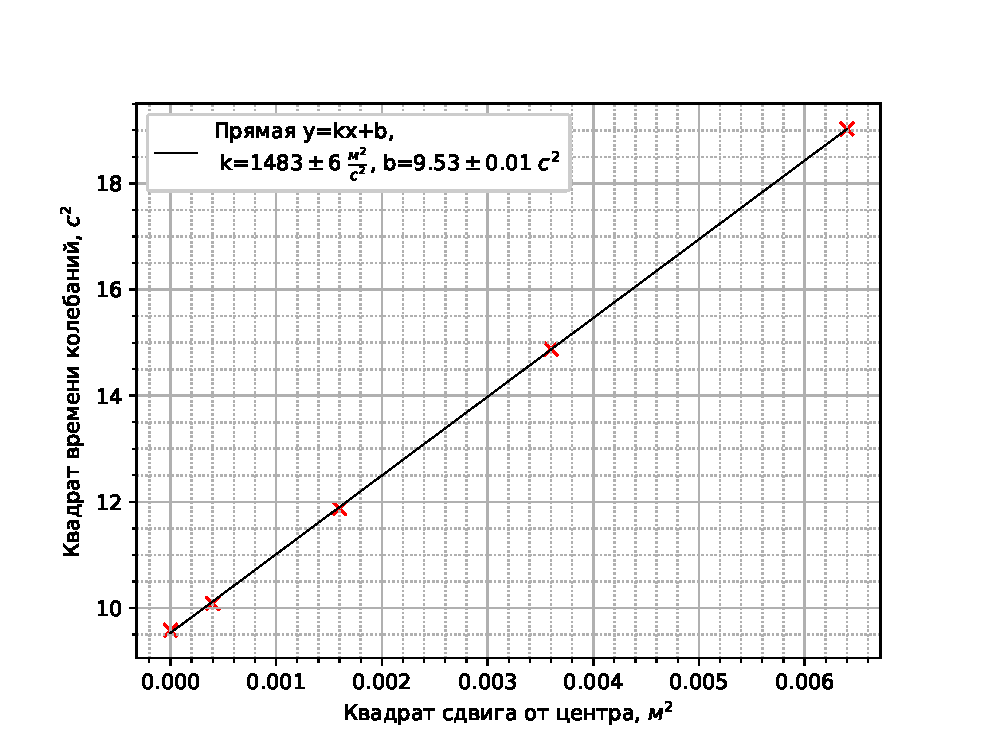
\includegraphics[width=\textwidth]{imgs/graph.eps}
    \caption{График зависимости $T^2(h^2)$}
    \label{fig:ust1}
\end{figure}

Посмотрим теоретическую зависимость по теореме Гюгенса-Штейнера

\begin{equation}
    2(I_{половинки}+m_{половинки}\cdot(h^2+r^2))=kmT^2
\end{equation}
, где $r$ - расстояние от центра полуокружности(фокуса) до чентра масс.

Тогда из графика мы получили, что $k_1=1483\pm6~\frac{м^2}{c^2}$.
И из предыдущей формулы получим

\begin{equation}
    m_{половинки}=\frac{m_{подвеса}kk_1}{2(1-kk_1)}
\end{equation}

Подставляя данные плучим $m_{половинки}=718\pm14$ г. Это значение практически совпадает со значением, измеренным напрямую $m_{половинки1}=720.7$ г и $m_{половинки1}=721.2$ г. А значит теорема Гюгенса-Штейнера выполняется.

\section{Выводы и обсуждения}
В данной работе был освоен метод измерения момента инерции с помощью трифилярного подвеса. Этот мем достаточно точный и позволяет с хорошей точностью определить момент инерции небольшого тела по одной из осей.

Были подтверждены ормулы для моментов инерции простых тел, а также сама аддитивность момента инерции.

Была доказана справедливость теоремы Гюгенса-Штейнера и найдена масса полуцилинров(сыров) с точнотью $2\%$.


\end{document}